\section{ViSTR-Bench}

\begin{figure}[!t]
  \centering
  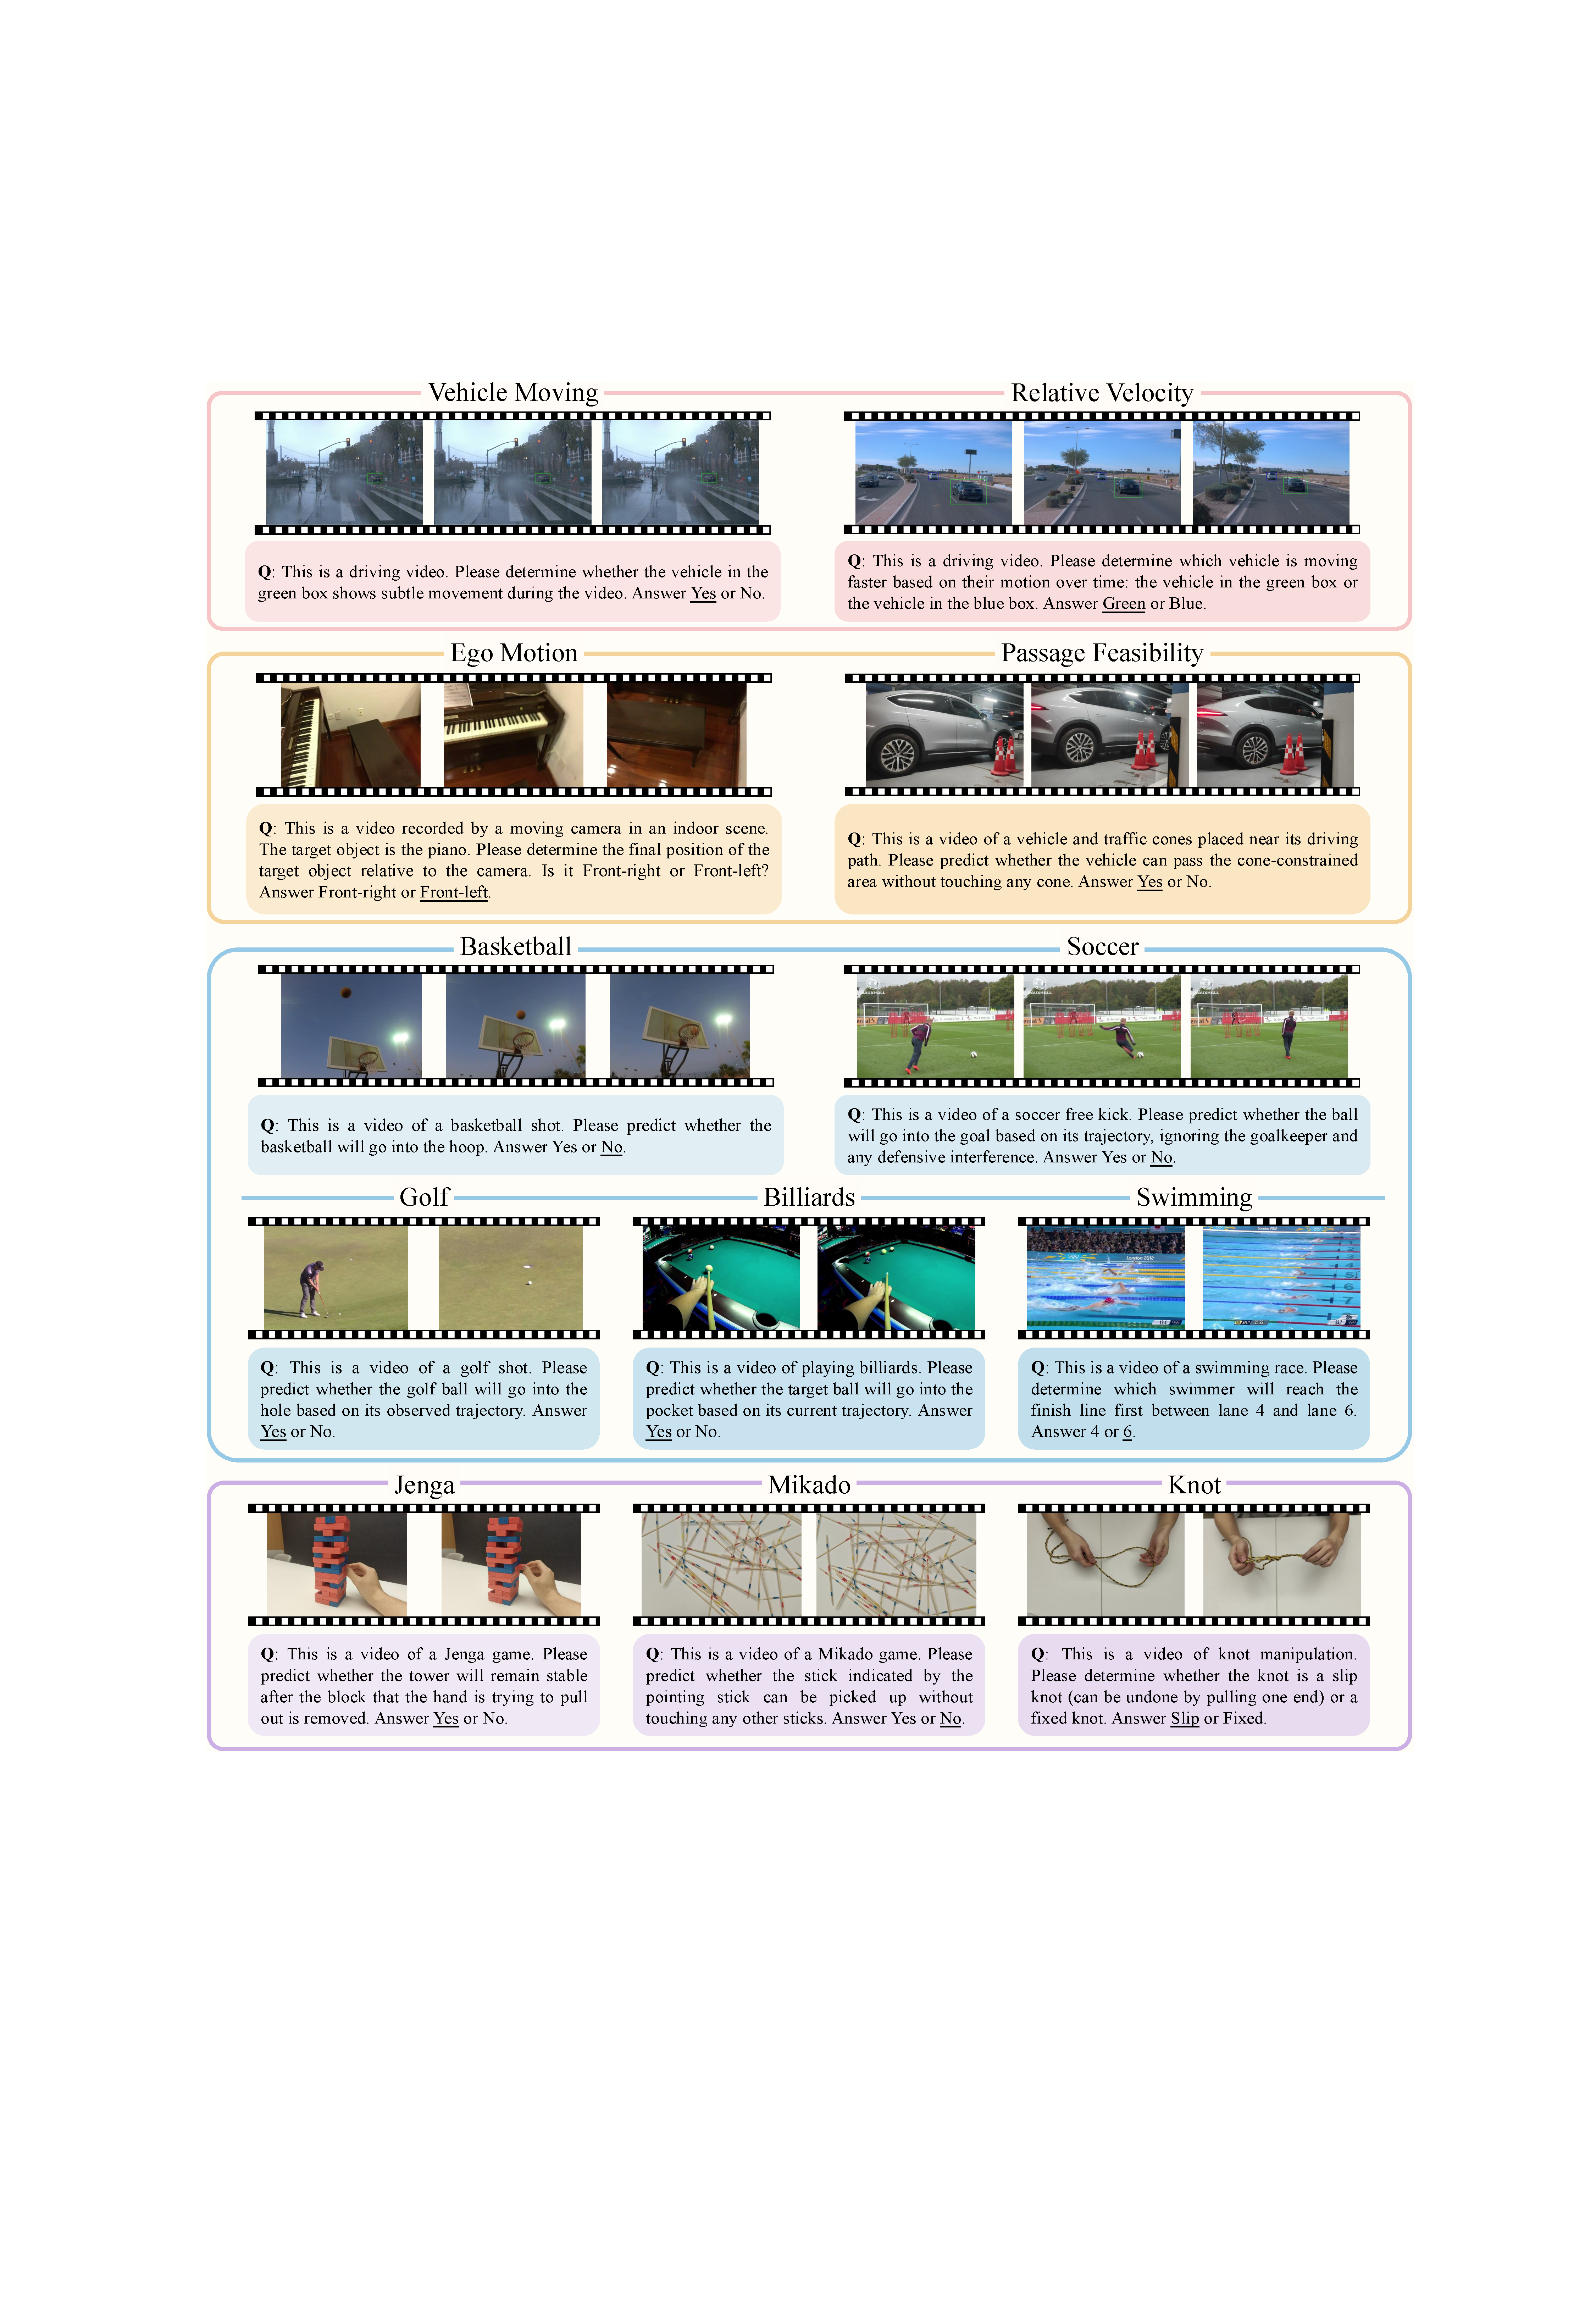
\includegraphics[height=0.70\textheight,keepaspectratio]{fig/fig_2.pdf}
  \caption{\textbf{Representative task examples from ViSTR-Bench.} Underlined options indicate the correct answers. Each task is formulated as a qualitative binary-choice question that requires models to aggregate temporal evidence and reason about dynamic visual scenes.}
  \label{fig:2}
\end{figure}

In this section, we first define the task taxonomy and reasoning objectives of ViSTR-Bench in Sec.~\ref{sec:task_definition}, and then describe the benchmark construction pipeline in Sec.~\ref{sec:benchmark_construction}.

\subsection{Task Definition}
\label{sec:task_definition}

ViSTR-Bench evaluates whether MLLMs can reason from continuous visual cues in dynamic scenes. Each task requires models to aggregate temporal evidence and make qualitative judgments about motion states, spatial relations, future outcomes, or latent physical properties. 
We organize ViSTR-Bench into four complementary dimensions, namely Motion Perception, Spatial Relations, Outcome Prediction, and Physical Dynamics, which comprise 12 subtasks in total. Representative task examples are shown in Figure~\ref{fig:2}, and the benchmark statistics are summarized in Figure~\ref{fig:3}.

\textbf{Motion Perception.}
This dimension evaluates whether MLLMs can perceive and compare object motion from continuous visual observations.
The core challenge is to distinguish true object motion from apparent visual changes caused by camera movement, viewpoint variation, or environmental distractors. 
\textit{Vehicle Movement} asks models to determine whether a target vehicle is actually moving over time. 
\textit{Relative Velocity} requires models to compare the speeds of two vehicles from an egocentric viewpoint. 
Both tasks test fundamental temporal perception abilities that cannot be reliably solved from a single static frame.

\textbf{Spatial Relations.}
This dimension focuses on reasoning about evolving spatial relationships and geometric constraints in dynamic scenes.
Unlike static spatial understanding, these tasks require models to account for camera motion, object positions, scene layout, and spatial clearance over time. 
\textit{Ego Motion} asks models to infer the spatial relationship between the observing camera and surrounding objects as the camera moves. 
\textit{Passage Feasibility} requires models to determine whether a vehicle can pass through a constrained passage without colliding with obstacles. 
These tasks emphasize observer-centric spatial reasoning and constraint-aware scene understanding.

\textbf{Outcome Prediction.}
This dimension evaluates whether MLLMs can infer future outcomes from historical motion cues before the final outcomes are directly observed. 
\textit{Basketball Shot}, \textit{Soccer Shot}, \textit{Golf Shot}, and \textit{Billiards Shot} require models to predict whether a moving object will reach a target based on its observed trajectory. 
\textit{Swimming Race} asks models to determine which swimmer will reach the finish line first from partial observations. 
These tasks require models to estimate motion trends, extrapolate trajectories, and reason about outcome-level consequences from temporal evidence.

\textbf{Physical Dynamics.}
This dimension examines whether MLLMs can reason about latent physical properties, dependencies, and stability conditions revealed through dynamic interactions. 
These properties are often ambiguous in static images but can be inferred as the physical process unfolds over time. 
\textit{Jenga Stability} requires models to predict whether a tower remains stable after block removal. 
\textit{Mikado Dependency} asks models to infer whether removing a target stick will disturb other sticks due to contact or support dependencies. 
\textit{Knot Type} requires models to identify the knot structure from its formation or manipulation process. 
These tasks go beyond visible motion and require inferring hidden physical states from temporal dynamics.

\begin{figure}[!t]
  \centering
  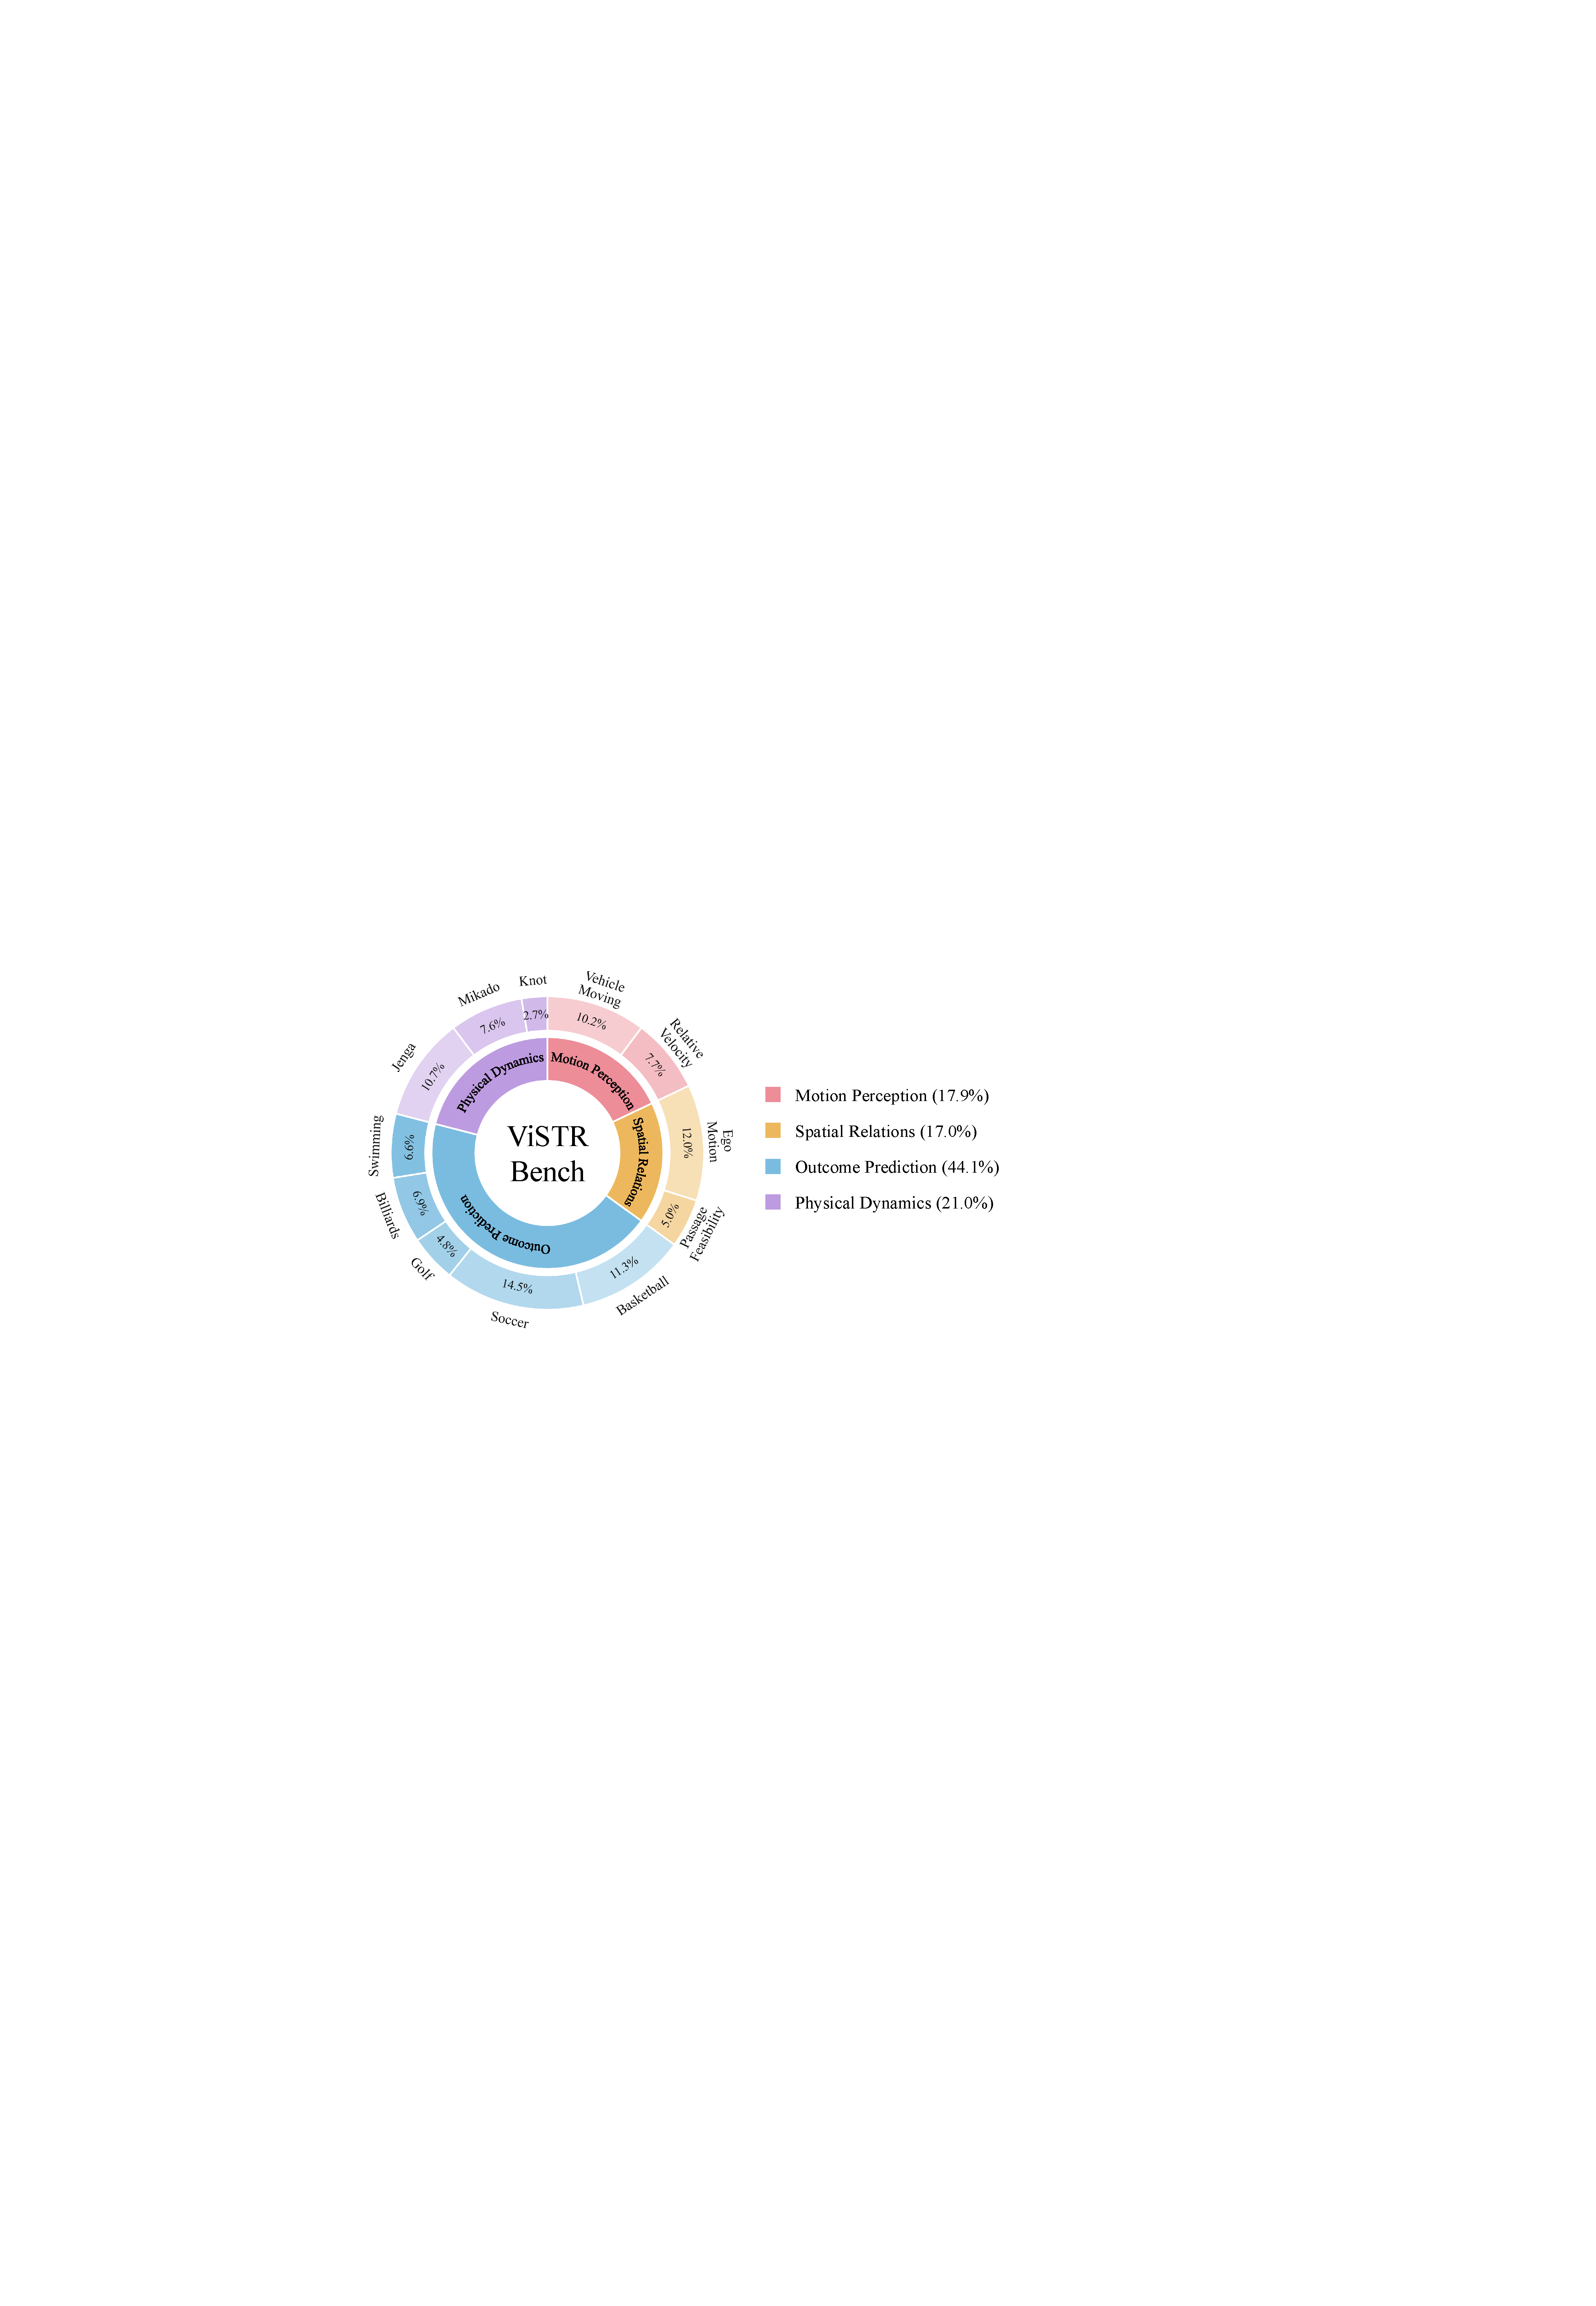
\includegraphics[width=0.60\linewidth]{fig/fig_3.pdf}
  \caption{\textbf{Benchmark statistics.} ViSTR-Bench consists of four task dimensions and 12 subtasks.}
  \label{fig:3}
\end{figure}

\subsection{Benchmark Construction}
\label{sec:benchmark_construction}

We construct ViSTR-Bench through a systematic multi-stage pipeline, including data collection, video preprocessing, question-answer (QA) pair generation, and human quality control, as shown in Figure~\ref{fig:4}. 
This pipeline is designed to ensure that each sample requires temporal evidence, supports high-level reasoning, and has an unambiguous qualitative answer.

\textbf{Data Collection.}
To cover diverse spatio-temporal reasoning scenarios across tabletop, indoor, and outdoor environments, we collect videos from established public datasets, curated web videos, and self-collected recordings.
Specifically, for autonomous driving scenarios, we sample videos from the Waymo Open Dataset~\citep{Waymo}. 
For indoor spatial reasoning, we use egocentric videos from ScanNet~\citep{ScanNet}, ScanNet++~\citep{ScanNet++}, and ARKitScenes~\citep{ARKitScenes}. 
For sports-related outcome prediction, we extract relevant clips from Ego4D~\citep{Ego4D} and further supplement them with web videos of corresponding sporting events. 
For specialized tasks that are difficult to construct from existing datasets, such as Passage Traversability and tabletop Physical Dynamics tasks, we conduct task-specific recordings in controlled real-world environments. 
Details of data sources are provided in Appendix~\ref{sec:detailed_data_sources}. 

\textbf{Video Preprocessing.}
Raw videos inherently contain multiple distinct events, irrelevant temporal context, and explicit outcomes that could trivialize reasoning tasks into simple recognition. 
To systematically eliminate these confounding factors and prevent shortcut learning by models, we process all collected videos through a three-stage preprocessing pipeline:
(1) \textbf{Event Localization.} 
To prevent the entanglement of multiple events and isolate specific reasoning instances, we localize raw videos into discrete, event-level clips and strip away unrelated temporal context.
(2) \textbf{Visual Prompting.} 
For object-centric tasks, textual descriptions alone may introduce referential ambiguity, especially in cluttered scenes with multiple similar objects. 
To explicitly ground target objects, we overlay visual markers (e.g., bounding boxes) onto the corresponding video frames. 
For instance, in the Vehicle Movement and Relative Velocity tasks, we leverage dataset annotations to highlight the specific vehicles in question.
(3) \textbf{Outcome Truncation.} 
For tasks in which the terminal outcome directly reveals the answer, we truncate videos before the outcome becomes visually explicit. 
Instead of using a fixed truncation ratio, we manually determine an instance-specific decision point for each clip, ensuring that the retained segment contains sufficient temporal evidence for human annotators to make a confident qualitative judgment. 
Collectively, these preprocessing steps standardize the visual inputs and mitigate confounding factors from irrelevant context, referential ambiguity, and answer-revealing frames.

\textbf{QA Pair Generation.}
We formulate all instances as binary-choice questions using task-specific templates. Detailed prompt templates are provided in Appendix~\ref{sec:detailed_prompt_templates}.
While most subtasks inherently follow a binary format, those with broader answer spaces, such as the Ego Motion task involving directions including front-left, front-right, back-left, and back-right, are converted to fit this framework. 
Specifically, we pair the ground-truth answer with a plausible distractor randomly sampled from the remaining valid options. To mitigate positional bias during model evaluation, the order of the two candidate options is systematically randomized for each question.

\textbf{Human Quality Control.}
To ensure the reliability of ViSTR-Bench, expert annotators manually filter all candidate QA pairs according to four strict criteria. 
Specifically, we first verify the \textit{visibility} of target objects, ensuring that they are identifiable based on either the textual description or visual prompts. 
We then examine the temporal \textit{sufficiency} of each clip to ensure that it contains adequate visual evidence for reasoning. 
Furthermore, we ensure the \textit{objectivity} of the dataset by requiring all ground-truth answers to be definitive and fully consistent with the observed visual events. 
Finally, we enforce a strict \textit{non-triviality} standard by discarding samples that can be trivially answered from a single static frame or by common-sense language priors. 
Through this rigorous review process, ViSTR-Bench establishes a reliable evaluation foundation for continuous spatio-temporal reasoning.

\begin{figure}[!t]
  \centering
  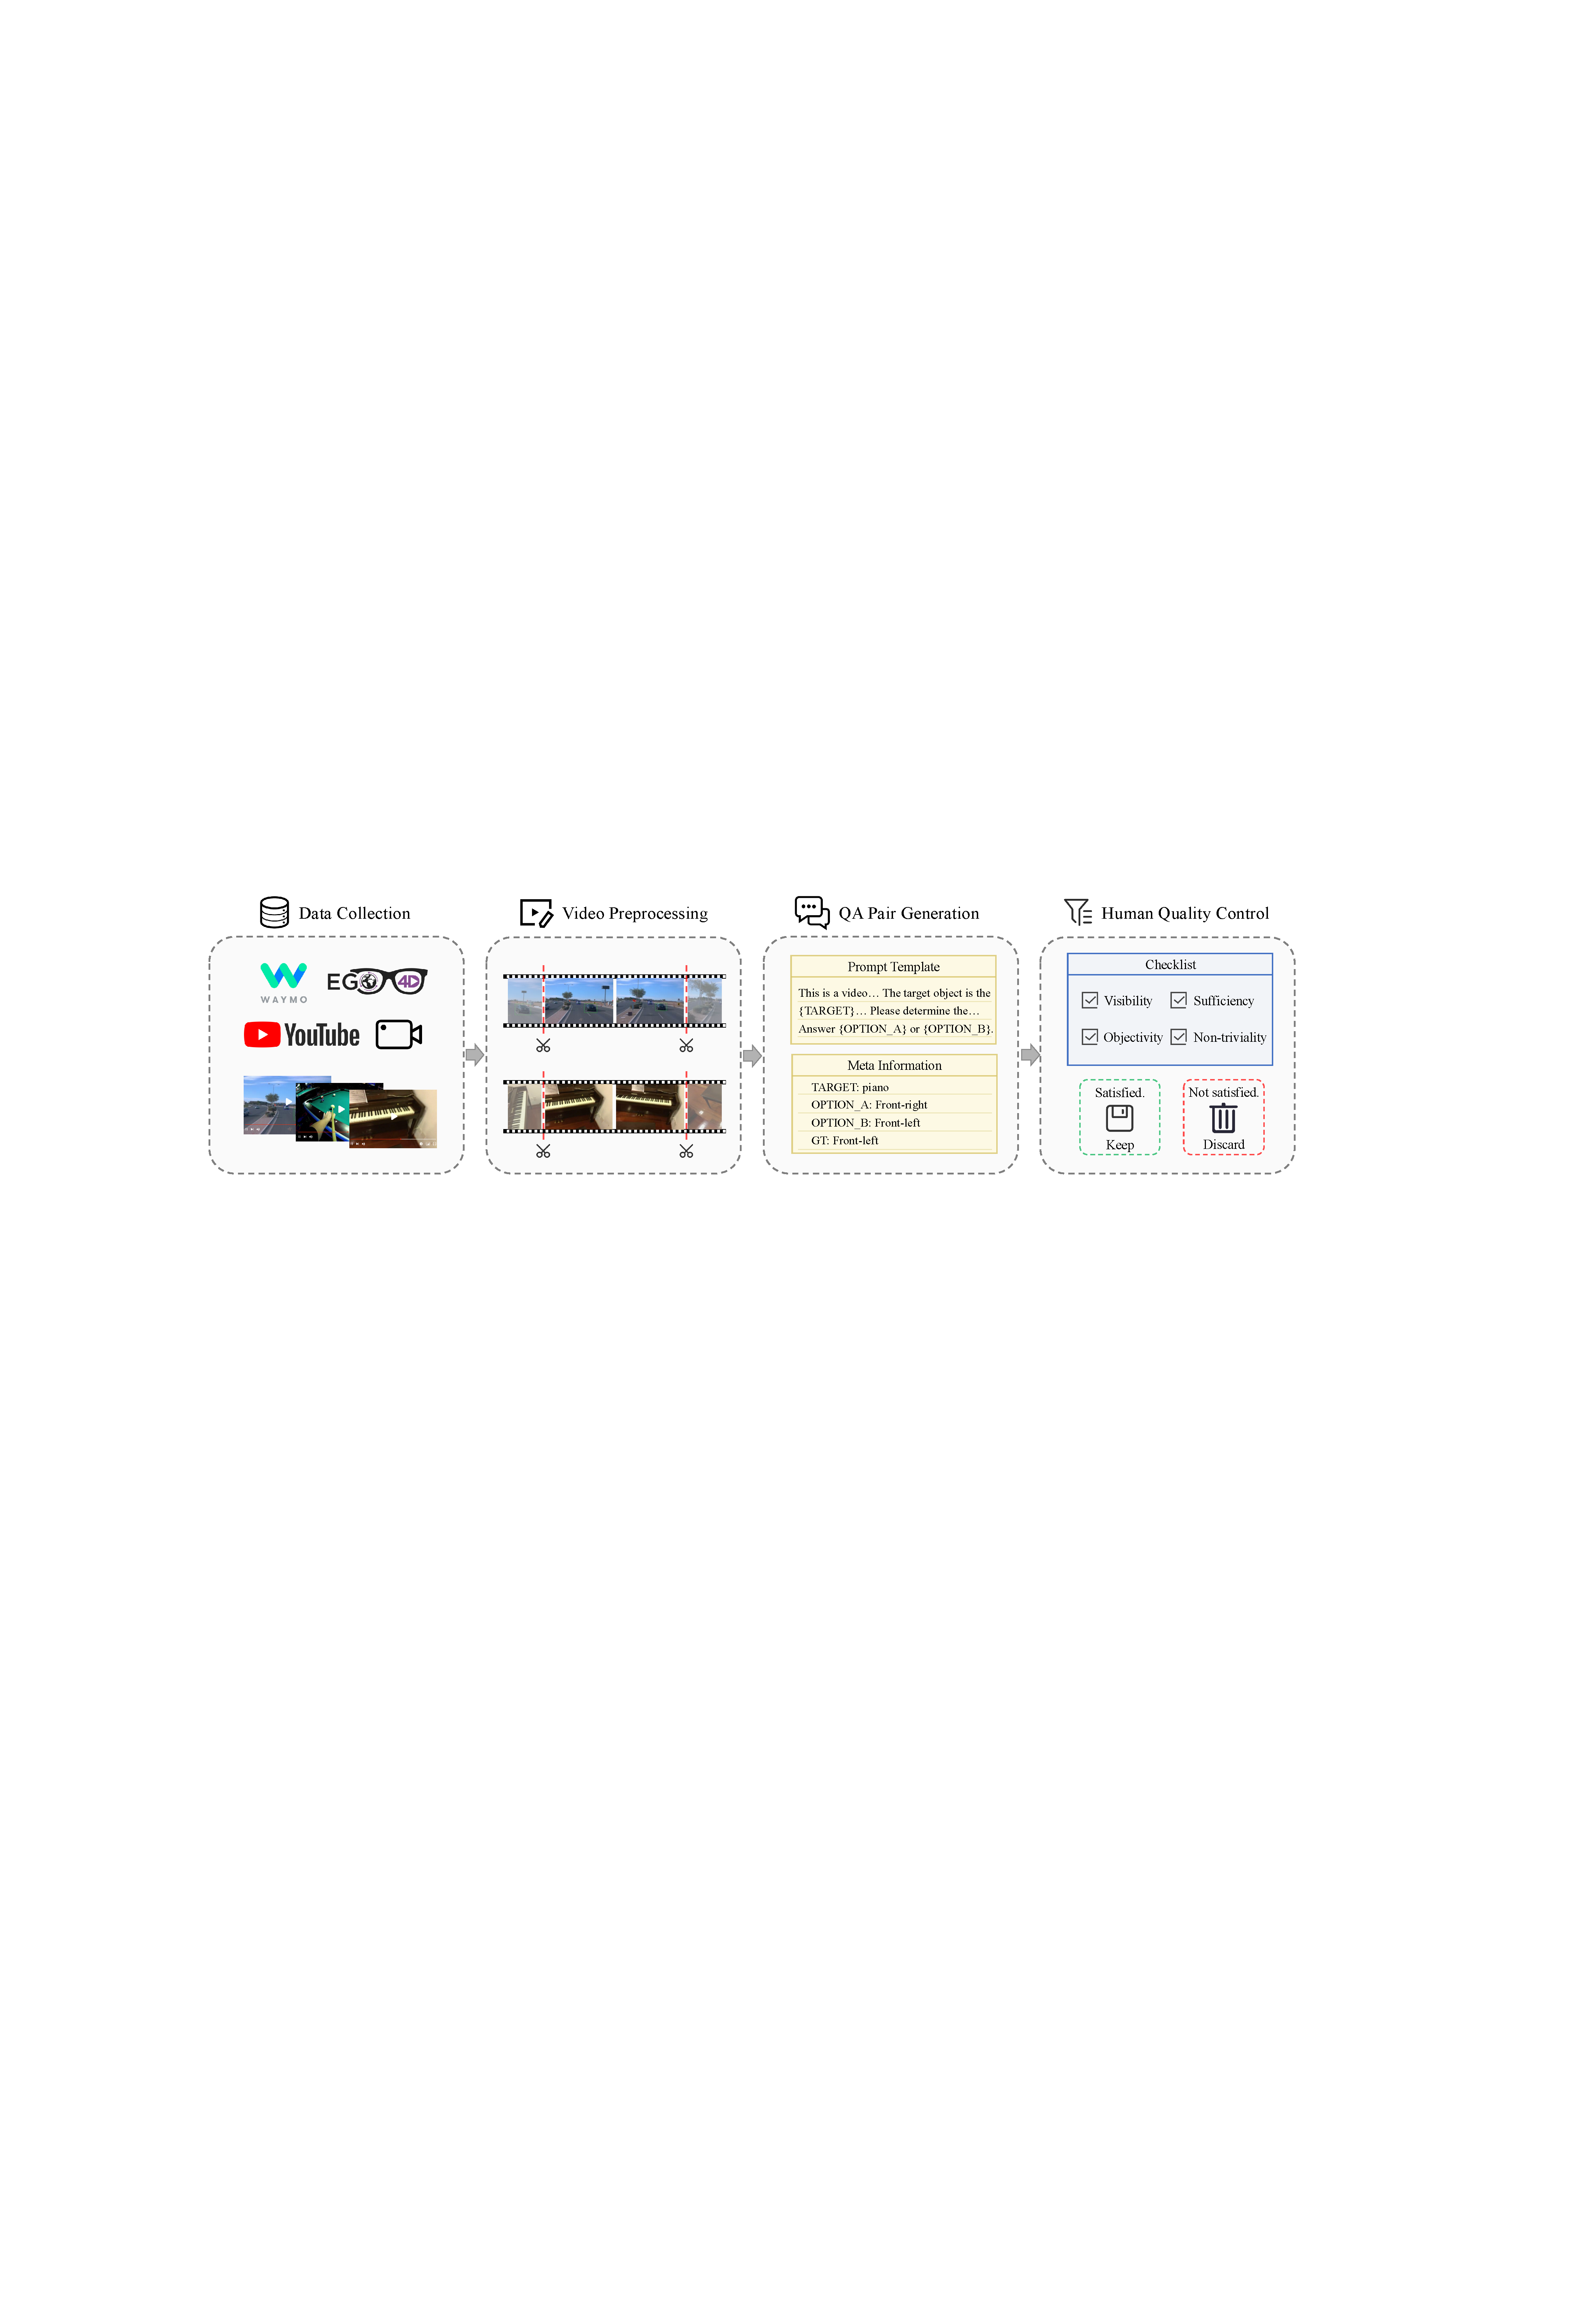
\includegraphics[width=0.95\linewidth]{fig/fig_4.pdf}
  \caption{\textbf{Benchmark construction pipeline.} We construct ViSTR-Bench through a systematic multi-stage process, including data collection, video preprocessing, QA pair generation, and human quality control. This pipeline ensures that each sample contains sufficient temporal evidence, supports high-level reasoning, and has an unambiguous qualitative answer.}
  \label{fig:4}
\end{figure}
